
%!TEX ROOT=ctutest.tex

\chapter{Rešerše}


\section{Podlahové vytápění}

U podlahového vytápění dochází k přenosu tepla do vytápěného prostoru převážně sáláním. Což má za následek, že se od sálající plochy ohřívají plochy osálané a teprve od sálajících a osálaných ploch se ohřívá okolní vzduch (druhá konvenkční složka z celkového tepelného toku). Naproti tomu při přenosu tepla pomocí deskových/článkových/trubkových otopných těles či konvektory dochází k přenosu pomocí proudění (konvekční složka). 
Teplota otopné plochy je poměrně nízká pohybuje se mezi 25 až 34~°C u podlahového vytápění a tedy i teplota teplonosné látky je nízká (otopná plocha je zahřívaná buď teplou vodou, teplým vzduchem nebo elektricky). Proto je tento typ vytápění vhodné využít při zapojení s nízkoteplotním zdrojem, jako jsou tepelná čerpadla, kondenzační kotle či solární panely.

Důležitým parametrem pro příjemný pobyt v místnosti je prostorové rozložení teploty, jak ve vertikální tak horizontální rovině. Na vertikální rozložení teplot ve vytápěné místnosti je způsobeno nerovnoměrným přívodem tepla a nerovnoměrným ochlazování jednotlivých stěn místnosti. Vertikální nerovnoměrnost teplot je tím větší, čím vyšší je povrchová teplota otopné plochy. Vzhledem k tomu, že teplota u podlahové vytápění je povrchová teplota otopné vody ze všech druhů velkoplošného vytápění (podlahové, stropní, stěnové) nejnižší, je vertikální rozložení teplot skoro ideální, viz obrázek \ref{fig:vertikalni-prubehy-teplot-pro-ruzne-druhy-vytapeni}a. Optimální vytápění by mělo zajistit, aby v oblasti hlavy stojícího člověka byla teplota minimálně o 2 °C nižší, než je v úrovni kotníků. Takovému ideálnímu průběhu teplot odpovídá obrázek \ref{fig:vertikalni-prubehy-teplot-pro-ruzne-druhy-vytapeni}b. Dále jsou na obrázku  \ref{fig:vertikalni-prubehy-teplot-pro-ruzne-druhy-vytapeni} další způsoby vytápění s vertikálními průběhy teplot. Na obrázku \ref{fig:porovnani-rozlozeni-teplot} je prostorové porovnání teplot podlahové vytápění a vytápění při využití deskových/článkových otopných těles s~vyznačenými oblastmi teplot.


\begin{figure}[h]

\centering
\begin{picture}(370,150)
\put(0,0){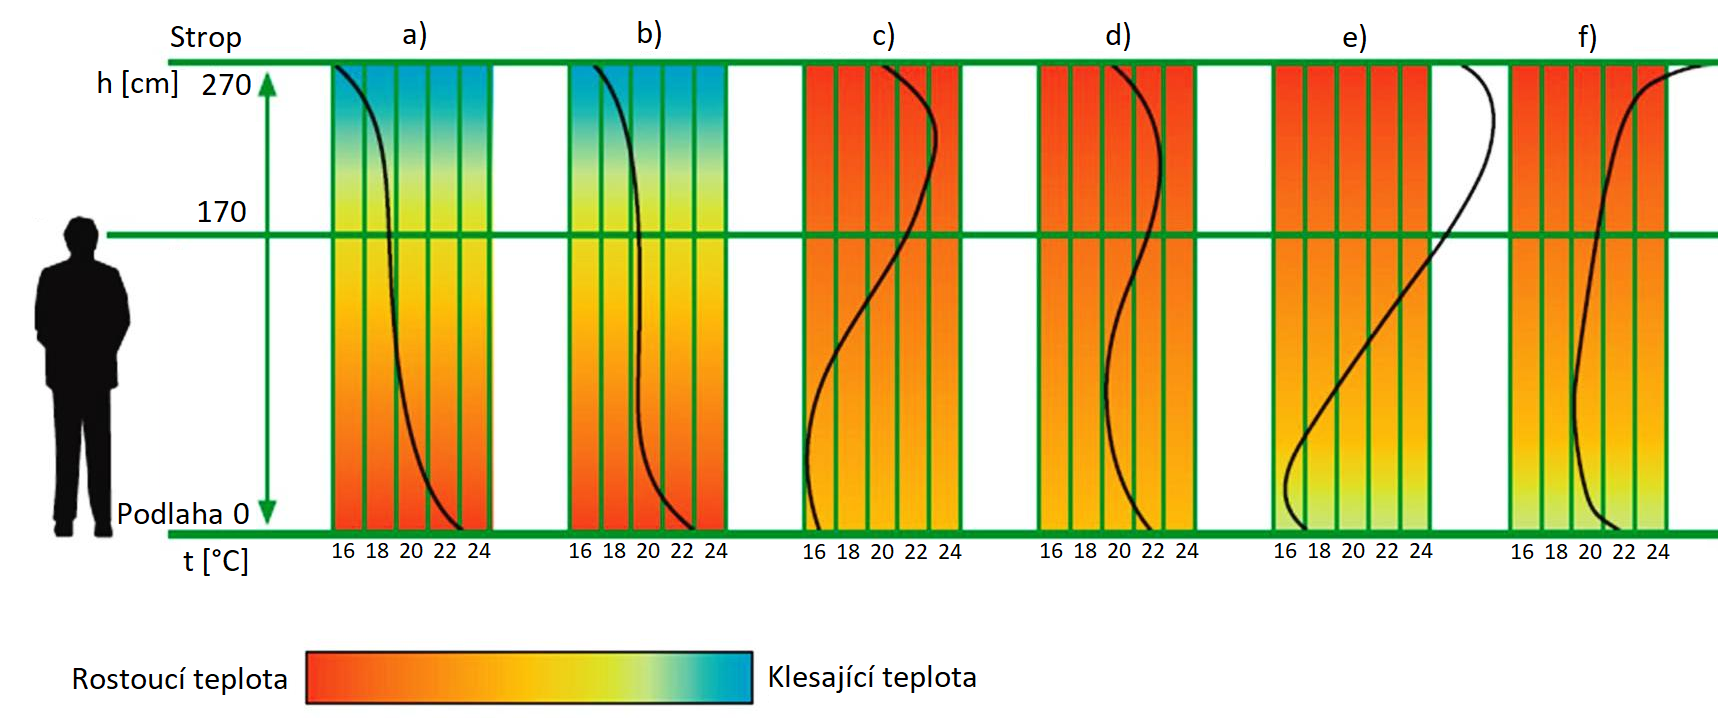
\includegraphics[width=\textwidth]{images/vertikalni-prubehy-teplot-pro-ruzne-druhy-vytapeni.png}}
\put(5,6){\scriptsize \sffamily Rostoucí teplota}
\put(161,6){\scriptsize \sffamily Klesající teplota}
\put(19,31){\scriptsize \sffamily t[°C]}
\put(15,132){\scriptsize \sffamily h[cm]}
\put(22,41){\fontsize{6}{6} \sffamily Podlaha}
\put(22,141){\fontsize{6}{6} \sffamily Strop}
\put(50,41){\scriptsize \sffamily 0}
\put(40,104){\scriptsize \sffamily 170}
\put(40,132){\scriptsize \sffamily 270}

\put(84,143){\scriptsize \sffamily a)}
\put(67,33){\fontsize{5}{5} \sffamily 16}
\put(74,33){\fontsize{5}{5} \sffamily 18}
\put(81,33){\fontsize{5}{5} \sffamily 20}
\put(88,33){\fontsize{5}{5} \sffamily 22}
\put(95,33){\fontsize{5}{5} \sffamily 24}

\put(134,143){\scriptsize \sffamily b)}
\put(117,33){\fontsize{5}{5} \sffamily 16}
\put(124,33){\fontsize{5}{5} \sffamily 18}
\put(131,33){\fontsize{5}{5} \sffamily 20}
\put(138,33){\fontsize{5}{5} \sffamily 22}
\put(145,33){\fontsize{5}{5} \sffamily 24}

\put(184,143){\scriptsize \sffamily c)}
\put(167,33){\fontsize{5}{5} \sffamily 16}
\put(174,33){\fontsize{5}{5} \sffamily 18}
\put(181,33){\fontsize{5}{5} \sffamily 20}
\put(188,33){\fontsize{5}{5} \sffamily 22}
\put(195,33){\fontsize{5}{5} \sffamily 24}

\put(234,143){\scriptsize \sffamily d)}
\put(217,33){\fontsize{5}{5} \sffamily 16}
\put(224,33){\fontsize{5}{5} \sffamily 18}
\put(231,33){\fontsize{5}{5} \sffamily 20}
\put(238,33){\fontsize{5}{5} \sffamily 22}
\put(245,33){\fontsize{5}{5} \sffamily 24}

\put(284,143){\scriptsize \sffamily e)}
\put(267,33){\fontsize{5}{5} \sffamily 16}
\put(274,33){\fontsize{5}{5} \sffamily 18}
\put(281,33){\fontsize{5}{5} \sffamily 20}
\put(288,33){\fontsize{5}{5} \sffamily 22}
\put(295,33){\fontsize{5}{5} \sffamily 24}

\put(334,143){\scriptsize \sffamily f)}
\put(317,33){\fontsize{5}{5} \sffamily 16}
\put(324,33){\fontsize{5}{5} \sffamily 18}
\put(331,33){\fontsize{5}{5} \sffamily 20}
\put(338,33){\fontsize{5}{5} \sffamily 22}
\put(345,33){\fontsize{5}{5} \sffamily 24}
\end{picture}
	 \caption[Vertikální průběh teploty vzduchu u podlahové vytápění.]{Vertikální průběh teploty vzduchu ve vytápěné místnosti při různém způsobu vytápění. \\ a) Ideální požadovaný průběh. b) Podlahové vytápění. c) Vytápění deskovými/článkovými otopnými tělesy (vnitřní stěna). d) Vytápění deskovými/článkovými otopnými tělesy (venkovní stěna). e) Konvektory. f) Stropní vytápění. Upraveno z \cite{vertikalni-prubehy-teplot-pro-ruzne-druhy-vytapeni}. }
	 \label{fig:vertikalni-prubehy-teplot-pro-ruzne-druhy-vytapeni}
\end{figure}

\hspace{5mm}

  \begin{figure}[H]
     \subfloat[Rozložení teplot při použití podlahové vytápění.\label{fig:rozlozeni-teplot-podlahove-vytapeni}]{
       \begin{overpic}[width=0.5\textwidth]{images/rozlozeni-teplot-podlahove-vytapeni.png}
         \put(20,10){\scriptsize \sffamily 22 °C}
         \put(65,50){\scriptsize \sffamily 20 °C}
         \put(8,115){\scriptsize \sffamily 17 °C}
         \put(155,90){\scriptsize \sffamily 18 °C}
       \end{overpic}
     }
     \subfloat[Rozložení teplot při použití deskových/článkových otopných těles. \label{fig:rozlozeni-teplot-radiatory}]{
       \begin{overpic}[width=0.5\textwidth]{images/rozlozeni-teplot-radiatory.png}
         \put(20,10){\scriptsize \sffamily 14 °C}
         \put(100,15){\scriptsize \sffamily 33 °C}
         \put(133,37){\scriptsize \sffamily 37 °C}
         \put(32,50){\scriptsize \sffamily 22 °C}
         \put(113,77){\scriptsize \sffamily 30 °C}
         \put(20,87){\scriptsize \sffamily 19 °C}
         \put(160,95){\scriptsize \sffamily 20 °C}
         \put(42,117){\scriptsize \sffamily 23 °C}
       \end{overpic}
     }
     \caption[Porovnání rozložení teplot při použití podlahové vytápění a~deskových/článkových otopných těles.]{Porovnání rozložení teplot při použití podlahové vytápění a deskových/článkových otopných těles. Upraveno z \cite{rozlozeni-teplot-podlahove-vytapeni-a-radiatory}.}\label{fig:porovnani-rozlozeni-teplot}
   \end{figure}
   


\subsubsection{Výhody}

\begin{itemize}
  \item Je vhodné zejména tam, kde je nízkoteplotní zdroj tepla (tepelné čerpadlo, kondenzační kotel, solární panely, …).
  \item Větší užitný prostor (místo nezabírají otopná tělesa).
  \item Cirkulace vzduchu je nižší oproti deskovým/článkovým otopným tělesům, proto je víření prachu v~místnosti menší.
  \item Téměř rovnoměrná teplota místnosti.
\end{itemize}

\subsubsection{Nevýhody}

\begin{itemize}
  \item Zvýšené náklady na realizaci.
  \item Nezbytná pečlivá montáž a stavební dozor.
  \item Vyšší tepelná setrvačnost otopné soustavy.
  \item Vyšší nároky na řízení podlahové otopné plochy (zejména hlídání maximální vstupní otopné vody).
\end{itemize}

\section{Zónová regulace vytápění}

Význam zónové regulace vytápění spočívá v systému umožňující individuální vytápění v~jednotlivých místnostech (každá místnost nebo spojení více místností se označuje za zónu) na požadovanou teplotu.  Základ zónové regulace je centrální řídicí jednotka, která přijímá data od jednotlivých místností (zejména jejich aktuální teplotu) a dává povely do zařízení, které ovládá (otevírání/zavírání pohonů u jednotlivých otopných okruhů apod.). Přístup k~řídicí jednotce je nejčastěji pomocí displeje, webového rozhraní nebo jejich kombinace. V řídicí jednotce se dá celý systém vytápění nastavit (nastavení časových a teplotních programů pro jednotlivé zóny a mnohé další). 

Zónové systémy vytápění se rozdělují na dvě hlavní skupiny. První tvoří zónové systémy propojené pomocí vodičů a druhou skupinu tvoří bezdrátová technologie propojující centrální řídicí jednotku a jednotlivé zóny. 

Hlavní částí zónového systému je centrální řídící jednotka. Mezi další komponenty patří, nástěnné snímače vnitřní teploty, snímač venkovní teploty, termoelektrické pohony, elektronické regulátory otopných těles, reléová spínací jednotka. Mezi komponenty, které přispívají ke komfortu zónové regulace jako senzor intenzity slunečního záření, senzor rychlosti větru, různé spínací jednotky, jednotky pro ovládání žaluzií, moduly pro dálkové ovládání pomocí GSM a další.

\subsection{Principy zónové regulace vytápění}

Jak již bylo řečeno, základem celého systému je centrální řídicí jednotka. Další důležitou částí je zónový regulátor, který slouží pro ovládání komponentů, které jsou k zónovému regulátoru připojeny. Mezi hlavní komponenty, který zónový regulátor ovládá, jsou termoelektrické pohony. Termoelektrický pohon je podobný termostatické hlavici, která se nasazuje na deskové/článkové otopné těleso, ale je jej možné ovládat elektrickým napětím. Samotná regulace vytápění probíhá tak, že řídicí jednotka je propojena se zónovým regulátorem. K~zónovému regulátoru jsou připojeny jednotlivé nástěnné snímače prostorové teploty a termoelektrické pohony, které jsou nasazeny na termostatický ventilech otopných okruhů/těles. V centrální jednotce jsou nastaveny časové programy (různé požadované teploty pro různé časové úseky). Centrální jednotka posílá do zónového regulátoru požadované teploty pro všechny zóny. Tyto  teploty jsou v zónovém regulátoru porovnávány s aktuálními prostorovými teplotami měřenými nástěnnými jednotkami. V případě, že je prostorová teplota příslušné zóny nižší než požadovaná teplota (nastavená v centrální jednotce), ovládá zónový regulátor odpovídající pohon, který otevírá/zavírá daný ventil a umožňuje proudění otopné vody do otopného okruhu/tělesa, čím dochází ke změně teploty v místnosti. Pokud je připojen například kotel, je pak hořák kotle ovládán při požadavku vytápění v jakékoliv místnosti. Princip zónové regulace je zobrazen na obrázku \ref{fig:obecny-princip-zonove-regulace}.

Další možné zapojení může být takové, že jednotlivé nástěnné snímače prostorové teploty jsou přímo propojeny s centrální jednotkou, která následně podle časového programu posílá zónovému regulátoru požadavky na ovládání jednotlivých pohonů. 

\newpage
\begin{figure}[H]
    \centering
    \def\svgwidth{\columnwidth}
    \input{images/svg/obecny-princip-zonove-regulace.pdf_tex}
    \caption{Obecný princip zónové regulace vytápění.}
    \label{fig:obecny-princip-zonove-regulace}
\end{figure}

Mezi další ovládaná zařízení při regulaci vytápění mohou být čerpadla, směšovací ventily zejména pro podlahové vytápění, kde je nutné udržovat teplotu otopné vody v daných mezích.

\subsection{Dostupné komerční řešení zónové regulace podlahového vytápění}

%Optimální systém pro otopnou soustavu, kterou hodlám řídit z obrázku~\ref{fig:otopna-soustava-rez-domu}, se skládá z řízení ovládání kotle, spínání čerpadel v případě zatopení v~krbech a~následnou indikaci uživateli, jak je moc zásobník otopné vody naakumulovaný, dále z jednotlivých otopných okruhů (12 pohonů pro 9 zón) a~čerpadla podlahového vytápění. Pro zónovou regulaci se používá pouze patro.

Na českém trhu se nachází poměrně velké množství výrobců se zařízeními pro ovládání podlahového vytápění. Snažil jsem se zaměřit hlavně na výrobce, které nabízejí drátové řešení. Výrobci však nabízejí kombinaci drátového a~bezdrátového řešení, především nástěnné snímače prostorové teploty jsou řešeny bezdrátově. Jedná se o modulový systém, který má být co nejvíce univerzální pro použití (především tam, kde se původně s~tímto typem řízení nepočítalo). Vybral jsem řešení od výrobců Elecktrobock, Honeywell a~Danfoss, jejichž řešení jsou popsány v textu níže.

Možná doplnit Loxon, icool jako něco na míru.


\subsubsection{Elektrobock}
Česká firma Elektrobock \cite{elektrobock-stranky} nabízí bezdrátové řešení pro řízení podlahové vytápění. Systém řízení je zastřešené pod aplikaci PocketHome \cite{pockethome-stranky}. Jednotlivé zařízení mohou fungovat samostatně bez nebo s centrální řídicí jednotkou. Tato centrální jednotka je zastřešené pod aplikaci PocketHome. Řídicí systém se skládá z centrální jednotky, nástěnných snímačů prostorové teploty pro jednotlivé místnosti a zónového regulátoru pro ovládání jednotlivých otopných okruhů a oběhového čerpadla, dále je k dispozici zařízení pro zapínání/vypínání kotle nebo komunikace pomocí protokolu OpenTherm. Na obrázku \ref{fig:elektrobock-pocket-home} jsou zobrazena jednotlivá zařízení. Komunikace je bezdrátová na frekvenci 433,92 MHz. Jednotlivé prvky mohou pracovat samostatně bez centrální jednotky, na druhou stranu se tímto ztrácí přehled o celém systému a komfortu nastavování z jednoho místa. Systém se může spravovat pomocí PC (systém Windows) nebo pomocí chytrého telefonu/tabletu (systém Android, iOS). Systém počítá s jedním zdrojem tepla, tedy kotlem (elektrickým, plynovým, automatickým), neuvažuje se s~otopnou soustavu, kde je začleněn např. krb s~tepelným výměníkem, jak z pohledu řízení čerpadel, tak i případnou indikaci o stavu naakumulovaní zásobníku s~otopnou vodou. Nástěnné snímače prostorové teploty jsou napájeny z baterií.


\begin{figure}[H]

\centering
\begin{picture}(370,250)
\put(0,0){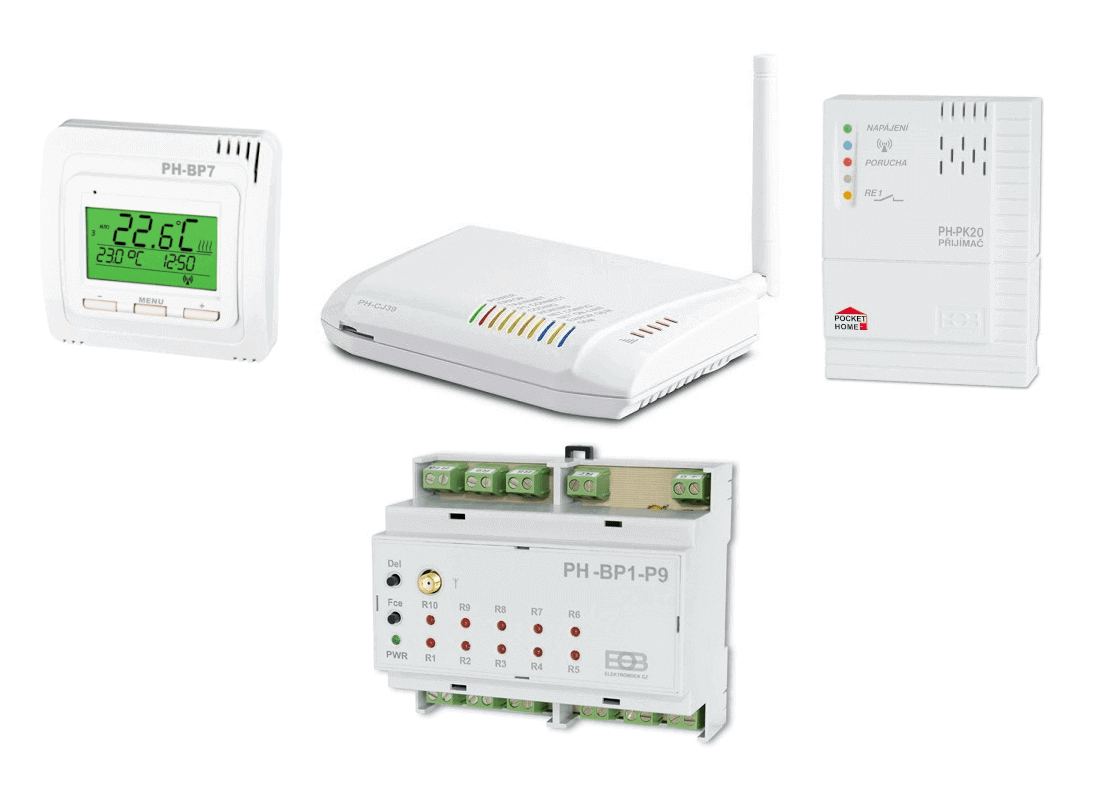
\includegraphics[width=\textwidth]{images/komercni-systemy/elektrobock-pocket-home/elektrobock-pocket-home.png}}
\put(50,226){\scriptsize \sffamily a)}
\put(180,190){\scriptsize \sffamily b)}
\put(305,235){\scriptsize \sffamily c)}
\put(180,8){\scriptsize \sffamily d)}
	 \caption[Jednotlivá zařízení systému Elektrobock PocketHome.]{Jednotlivá zařízení systému Elektrobock PocketHome. \\ 
	 a) Nástěnný snímač prostorové teploty. b) Centrální jednotka. c) Spínací jednotka kotle. d) Zónový regulátor. Upraveno z \cite{elektrobock-lokalni-termostat, elektrobock-centralni-jednotka, elektrobock-spinaci-jednotka-kotle, elektrobock-zonovy-regulator}.}
	 \label{fig:elektrobock-pocket-home}
\end{picture}

\end{figure}

\subsubsection{Honeywell}
Honeywell nabízí bezdrátový systém regulace podlahové vytápění. Systém řízení je zastřešené pod aplikaci Evohome \cite{honeywell-evohome-stranky}. Skládá se z centrální jednotky s~dotykovým displejem, nástěnných snímačů prostorové teploty pro jednotlivé místnosti, zónového regulátoru pro ovládání jednotlivých otopných okruhůš. Systém je možné rozšířit o dobíjení \acrshort{tuv} (\textit{\acrlong{tuv}}), pro sledování teploty na zásobníku je možné umístit teplotní čidlo, ze kterého je teplota odesílaná do centrální jednotky. Na obrázku \ref{fig:honeywell-evohome} jsou zobrazena jednotlivá zařízení systému. Systém však při dobíjení zásobníku TUV počítá se zdrojem tepla pouze s kotlem, takže v případě využití krbů s výměníkem nastává problém. V neposlední řadě umožňuje zapojit směšovací ventil pro optimální teplotu do podlahového topení. Systém je možné ovládat lokálně nebo řídit vzdáleně odkudkoliv, je zapotřebí zaregistrovat si účet a spárovat ho s  centrální jednotkou. Vzdálený server přijímá požadavky na změny režimů či nastavení teplot, a zasílá je do řídící jednotky. Server průběžně shromažďuje různá data o chování soustavy, a může je na základě žádosti poskytnout. Z~toho vyplývá, že pro lepší řízení a nastavení vytápění je nutné zřídit vzdálený přístup a samotné vyhodnocení a dání povelů, pak dochází na vzdálením serveru, nemáme moc pod kontrolou data a životnost takového systému do budoucnosti. Otázka je i při využití pouze lokálního režimu, zda regulace nepřichází o~výhody cloudového řešení. Komunikace mezi zařízeními probíhá na frekvenci 868 MHz, připojení k centrální jednotce pomocí mobilní aplikace je pomocí WiFi. Nástěnné snímače prostorové teploty a řízení dobíjení TUV jsou napájeny z baterií.

\newpage

\begin{figure}[H]

\centering
\begin{picture}(370,300)
\put(0,0){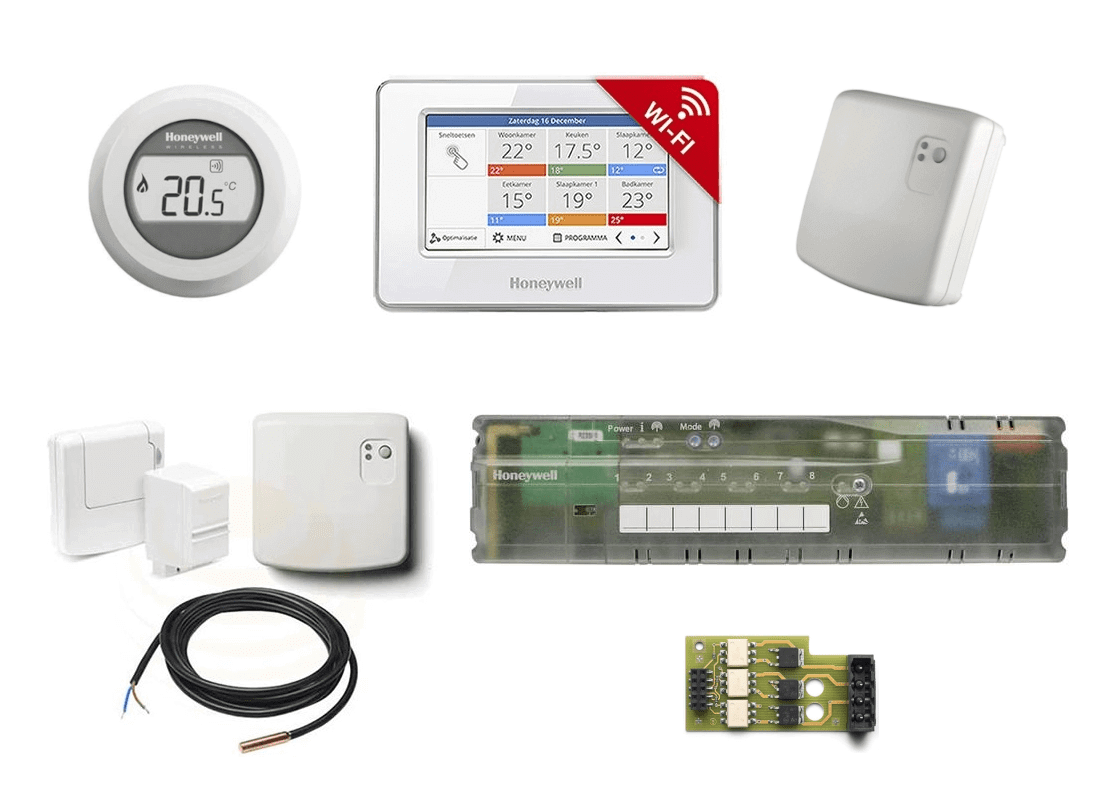
\includegraphics[width=\textwidth]{images/komercni-systemy/honeywell-evohome/honeywell-evohome.png}}
\put(60,240){\scriptsize \sffamily a)}
\put(180,240){\scriptsize \sffamily b)}
\put(305,240){\scriptsize \sffamily c)}
\put(60,130){\scriptsize \sffamily d)}
\put(250,130){\scriptsize \sffamily e)}
\put(250,57){\scriptsize \sffamily f)}
	 \caption[Jednotlivá zařízení systému Honeywell Evohome.]{Jednotlivá zařízení systému Honeywell Evohome.  \\
	 a) Nástěnný snímač prostorové teploty. b) Centrální jednotka. c) Spínací jednotka kotle. d) Řízení dobíjení TUV. e) Zónový regulátor. f) Rozšiřující modul pro  zónový regulátor. Upraveno z \cite{honeywell-lokalni-termostat, honeywell-centralni-jednotka, honeywell-spinaci-jednotka-kotle, honeywell-rizeni-dobijeni-tuv, honeywell-zonovy-regulator, honeywell-rozsirujici-modul-pro-zonovy-regulator}.}
	 \label{fig:honeywell-evohome}
\end{picture}

\end{figure}

\subsubsection{Danfoss}
Danfoss nabízí bezdrátový systém regulace podlahové vytápění. Systém řízení je zastřešený pod aplikaci Danfoss Link \cite{danfoss-link}. Řídicí systém se skládá z centrální jednotky s dotykovým displejem, nástěnných snímačů prostorové teploty  pro jednotlivé místnosti a zónového regulátoru pro ovládání jednotlivých otopných okruhů, oběhového čerpadla a řízení kotle. Na obrázku \ref{fig:danfoss-danfoss-link} jsou zobrazena jednotlivá zařízení systému. Vzdálené ovládání je umožněno přes mobilní aplikací pomocí cloudového řešení. Systém má absenci v řízení dobíjení TUV, respektive zásobníku na otopnou vodu a použití více zdrojů tepla (viz předchozích systémy). Komunikace mezi zařízeními probíhá na frekvenci 868~MHz. Nástěnné snímače prostorové teploty jsou napájeny z baterií.

\begin{figure}[H]
\centering
\begin{picture}(370,250)
\put(0,0){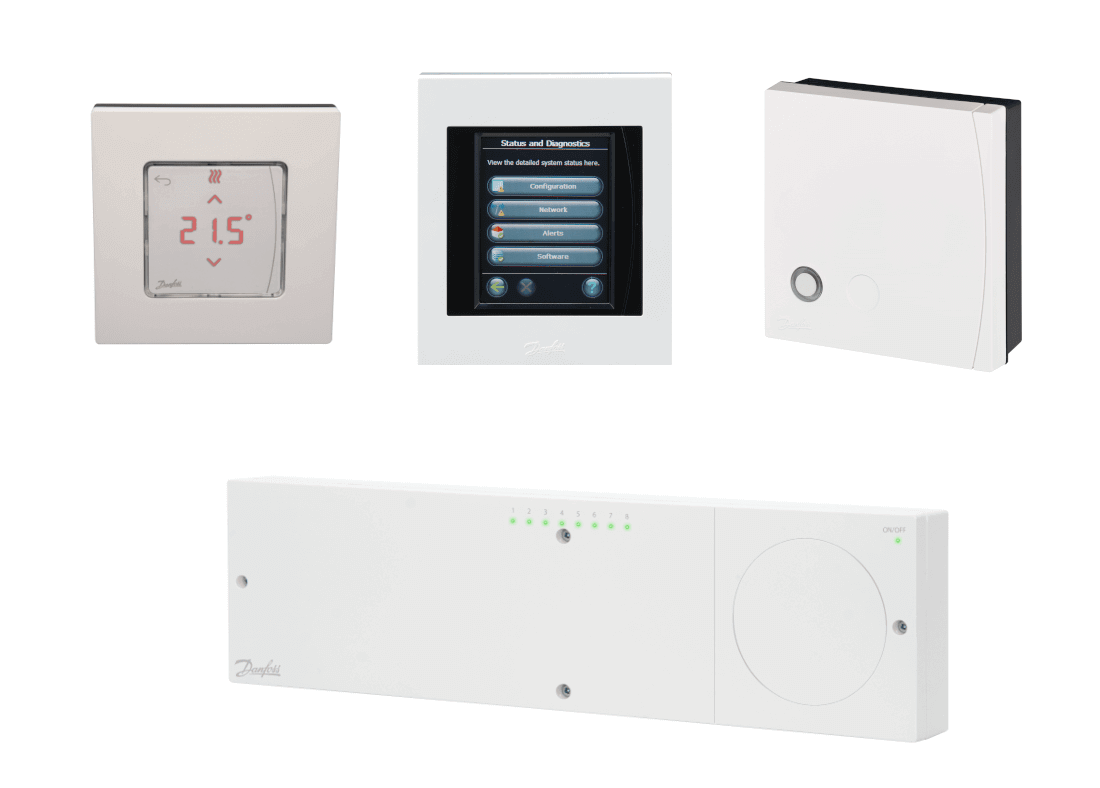
\includegraphics[width=\textwidth]{images/komercni-systemy/danfoss-danfoss-link/danfoss-danfoss-link.png}}
\put(60,242){\scriptsize \sffamily a)}
\put(180,242){\scriptsize \sffamily b)}
\put(305,242){\scriptsize \sffamily c)}
\put(180,102){\scriptsize \sffamily d)}
	 \caption[Jednotlivá zařízení systému Danfoss Danfoss Link.]{Jednotlivá zařízení systému Danfoss Danfoss Link. \\
	 a) Nástěnný snímač prostorové teploty. b) Centrální jednotka. c) Spínací jednotka kotle. d) Zónový regulátor. Upraveno z \cite{danfoss-lokalni-termostat, danfoss-centralni-jednotka, danfoss-zonovy-regulator, danfoss-spinaci-jednotka-kotle}.}
	 \label{fig:danfoss-danfoss-link}
\end{picture}

\end{figure}

Pokud shrnu hlavní nedostatky zmíněných systémů pro řízení podlahového vytápění, tak mezi ně patří bezdrátové ovládání, zejména tedy možný problém komunikace mezi centrální jednotkou a zařízeními. Výměna baterií v~zařízeních po určité době. Dále absence počítání s více zdroji tepla a~centrálním zásobníkem otopné vody, systém od firmy Honeywell umožňuje ovládaní ohřev pro TUV. Dalším možným nedostatkem může být cloudové řešení z pohledu dlouhodobé garance fungování služby, dále pak vzdálené ovládání neprobíhá přímo s centrální jednotkou, ale se vzdáleným serverem. Další zjištěním bylo, že všechny systémy jsou nabízeny jako bezdrátové, což je samozřejmě pochopitelné jak z pohledu jednoduchého nainstalování, již do stávajících staveb, kde s takovým systémem nebylo počítáno (zejména staré zástavby), též není nutné provádět žádné stavební úpravy. Pokud jsou nabízena drátová řešení není zde žádná centrální jednotka, ovládání probíhá přes drátové nástěnné snímače prostorové teploty připojené přímo na zónový regulátor, který následně ovládá jednotlivé otopné okruhy. Celkový počet  zařízení nutných pro ovládání vytápění rodinného domu (jehož dispozice jsou popsány v textu níže, část \ref{sec:popis-celkoveho-konceptu}) shrnuje tabulka \ref{tab:srovnani-vlastnosti-jednotlivych-komercnich-systemu}, zobrazuje přehled funkcí systémů zmíněné výše.


\begin{center}
\begin{table}[H]
\begin{threeparttable}
\begin{tabular}{|c||c|c|c|} \hline
\backslashbox{Funkce}{Systém}
& \thead{Elektrobock \\ (PocketHome)}  & \thead{Honeywell \\ (Evohome)} & \thead{Danfoss \\ (Danfoss Link)} \\


\hline
\thead{Napojení na více \\ zdrojů tepla} & Ne & Ne & Ne \\ 
\hline
\thead{Napojení na \\ centrální zásobník \\ otopné vody} & \multirow{2}{*}{Ne} & \multirow{2}{*}{Ne} & \multirow{2}{*}{Ne} \\ 
\hline
\thead{Ohřev TUV} & Ne & Ano & Ne \\ 
\hline
\thead{Bezdrátové$\slash$drátové \\ řešení} & Bezdrátové & Bezdrátové & Bezdrátové \\ 
\hline
\thead{Možnosti ovládání} & \makecell{PC \\ chytrý telefon} & \makecell{dotykový displej \\ chytrý telefon } & chytrý telefon \\ 
\hline
\thead{Cloudové řešení} & Ne & Ano & Ano \\ 
\hline
\makecell{Centrální \\ řídicí jednotka} & \makecell{(PH-CJ39-WIFI, 1×) \\ 3\,678 Kč}  & \makecell{(ATC928G3026,  1×) \\ 5\,994 Kč } & \makecell{(014G0288, 1×) \\ 8\,694 Kč }\\
Zónový regulátor & \makecell{(PH-BP1-P9, 2×) \\ 3\,388 Kč} & \makecell{(HCE80, 2×) \\ 5\,622 Kč} & \makecell{(088U1031, 2×) \\ 4\,299 Kč} \\
\makecell{Nástěnný snímač \\ prostorové teploty} & \makecell{(PH-BP7-V, 13×) \\ 9\,036 Kč} & \makecell{(T87RF2083, 13×) \\ 12\,141 Kč} & \makecell{(088U1081, 13×) \\ 19\,476 Kč} \\
Spínací jednotka kotle & \makecell{(PH-PK20, 1×) \\ 1\,498 Kč} & \makecell{(BDR91A1000, 1×) \\ 1\,100 Kč} & \makecell{(014G0272, 1×) \\ 2\,190 Kč}\\
Řízení dobíjení TUV & -- & \makecell{(ATF500DHW, 1×) \\ 3\,818 K}  & -- \\
\makecell{Rozšiřující modul \\ pro zónový regulátor}  & -- & \makecell{(HCS80, 1×) \\ 1 897 Kč} & -- \\
\thead{Celková cena \\ včetně DPH \tnote{a}} & 25\,004 Kč & 41\,590 Kč & 47\,614 Kč\\ 
\hline
\end{tabular}

	\begin{tablenotes}
    	\item[a] Ceny stanoveny ke dni 26. 11. 2020.
	\end{tablenotes}

\end{threeparttable}
 \caption{Srovnání funkcí jednotlivých komerčních systémů.}
 \label{tab:srovnani-vlastnosti-jednotlivych-komercnich-systemu}
 
\end{table}
\end{center}

V tabulce \ref{tab:srovnani-vlastnosti-jednotlivych-komercnich-systemu} chybí pohony pro ovládání jednotlivých otopných okruhů pomocí zónového regulátoru. Pro výše zmíněné systémy, zónový regulátor podporuje pohony na 230 V AC, pohony je možné koupit  přímo od daného výrobce nebo od jiného, na samotnou funkčnost to nemá vliv. Jediný rozdíl může být v pořizovací ceně, kde pro termoelektrické pohony je cena od 400 do 800 Kč, pro servopohony může být cena ještě vyšší. Celková cena za 24 pohonů (pro dvě patra) se pohybuje v řádu jednotek tisíc. Někteří výrobci jako Danfoss nabízejí v případě špatného dosahu signálu opakovače, ale je nutné počítat s dalšími náklady navíc (řády jednotek tisíc). V případě, že systém neumí ovládat kotel pro dobíjení TUV, případně nesplňuje požadavky, které bychom chtěli, pak je nutné využít jiné řešení/systém, což se dále promítá do dalších nákladů a hlavně se jedná o nejednotnost jednoho systému.







